\documentclass[openany]{book}
\usepackage[utf8]{inputenc}
\usepackage{fullpage}
\usepackage{float}
\usepackage{graphics}
\usepackage{graphicx}
\usepackage{csquotes}
\usepackage{hyperref}
\usepackage{amsmath}
\usepackage{tikz}
\usepackage{pgfplots}
\usepackage{tikz-3dplot}
\usepackage{import}
\usepackage{color}
\usepackage{amssymb}
\usepackage{epstopdf}
\usepackage{bold-extra}
\usepackage{caption}
\usepackage{subcaption}
\usepackage[T1]{fontenc}
\usepackage{xargs}
\usepackage{etoolbox}

\bibliographystyle{unsrt} 

\setlength\parindent{0pt}

\begin{document}
	


		\begin{titlepage}
		\centering
		
		{\Huge Astrophysical S-factor calculation for selected reactions  \par}
		
		\begin{figure}[H]
			\centering
			
\includegraphics[width=0.5\linewidth]{logo.pdf}
			\label{fig:logo}
		\end{figure}
		{\Large Author:  \par}
		{\Large Carlos Alberto Calvachi Salas \par}
		{\Large 201822667 \par}
		\vfill
		{\Large\textit{Final project submitted in partial fulfillment of the requirements for the degree of} \par}
		\vfill
		{\Large\textit{Physicist} \par}
		\vfill
		{\Large Advisor:  \par}
		{\Large Neelima Govind Kelkar Ph.D. \par}
		\vfill
		{\Large Universidad de los Andes  \par}
		{\Large Physics Department  \par}
		{\Large December, 2022  \par}
		{\Large Bogotá, Colombia \par}
	\end{titlepage}

\chapter*{Abstract}

Review on relevant elements of nuclear astrophysics. \\

Definition, motivation and applications of the astrophysical S-factor. \\

Survey on models that predict S-factors. They are mainly classified as empirical, potential, macroscopic and matrix models \\

Use of theoretical models to calculate the S-factors of selected reactions. \\

Comment on the applicability of the models for each reaction. Comparison between experimental data and theoretical predictions of the S-factors.

\clearpage

\chapter*{Acknowledgments}

Mom for everything.

\clearpage

\tableofcontents
\listoffigures
\listoftables

\newcommand{\reaction}[8]{
	
	\mathrm{{}^{#1}#2({}^{#3}#4, {}^{#5}#6){}^{#7}#8 }

}


\newcommand{\graph}[3]{
	
\begin{figure}[H]
	\centering
	\includegraphics{Graphs/#1.eps}
	\caption[#2]{#3}
	\label{fig:#1}
\end{figure}

}

\newcommand{\radiativeCapture}[1][p]{
	(#1, \gamma)
}

\newcommandx*{\Cfusion}[2][1=12, 2=12]{
	\mathrm{C{}^{#1} +  C{}^{#2}}
}

\newcommandx*{\Ofusion}[2][1=16, 2=16]{
	\mathrm{O{}^{#1} +  O{}^{#2}}
}


\chapter{Nuclear astrophysics fundamentals}  \label{ch:nuclearAstrophysics}

In order to apply nuclear astrophysics to the study of star element production, there are essentials to be considered. In this chapter, a general review of the main points relevant for nuclear physics are presented that emphasizes selected topics that are relevant in the field of nuclear astrophysics.

\section{General aspects about the nucleus} \label{sec:nucleiAspects}
Introduce a brief description of the nuclei.
\indent The structure of the nuclei
\indent The nuclear models

The nucleus is a bound state of a system of protons and neutrons. These substructures are bound states of a set of fundamental particles, which are called quarks.  \\

A general treatment given in \cite{basdevant_rich_spiro_2004} and basic concepts in \cite{heyde_2020}. \\

A more particular on nuclear astrophysics \cite{iliadis_2015}. \\

Rest energy.

\begin{equation} \label{eq:restEnergy}
	E_0 = Zm_pc^2 + (A-Z)m_nc^2 - B(A, Z),
\end{equation}

where $Z$, $A$ are the atomic and mass number respectively. 

\tdplotsetmaincoords{60}{155}
\pgfplotsset{compat=newest}

\begin{tikzpicture}[tdplot_main_coords, scale = 5]


\shade[ball color = red,
opacity = 1.0
] (-0.05,0,0) circle (0.11em);

\shade[ball color = black,
opacity = 1.0
] (0.05,0,0) circle (0.11em);

\shade[ball color = red,
opacity = 1.0
] (0,0,0) circle (0.11em);

\shade[ball color = black,
opacity = 1.0
] (0,0.05,0) circle (0.11em);


\shade[ball color = black,
opacity = 1.0
] (0,0,0.05) circle (0.11em);

\shade[ball color = red,
opacity = 1.0
] (0,0.05,0.05) circle (0.11em);

 %\node[circle,draw, color=yellow] (c) at (1,1,1){}; 



\end{tikzpicture}

\usetikzlibrary {arrows.meta,bending,positioning} 
\begin{tikzpicture}
	\draw [-{Stealth}, decorate, decoration=snake] (1, 0) -- (3,2) 
	node [right] {$\gamma$} ;
	\draw[{Stealth[blue]}-{Stealth[blue]}] (0,0.3) -- (1,0.3);
\end{tikzpicture}

Each nucleus is compound of a finite number of proton and neutrons. In addition, 

Elementary nuclear structure 
-	Atomic nuclei are bond states of nucleons 
They are particles
Characteristics 
-	They obey the Pauli-exclusion principle like electrons
- 	They have magnetic moment.
-	They are bonded in the nuclei by the strong force which compensates the repulsive electromagnetic force
-	Each nucleon is conformed by elementary particles.
Classification 
-	proton: positive charge
-	neutron: no charge  

-	Mass number. Atomic number.

Leptons 
Characteristics
-	They do not interact via strong force
-	Considerably lighter in mass than nucleons
Classification 
-	Electron 
-	Neutrino 
-	Antiparticles are also considered

%\section{Interactions}
%\subsection{Electromagnetic interaction}
%Electromagnetic transitions.
%\subsection{Strong interaction}
%Interaction 
%-	The Yukawa potential. 

%\begin{equation}
%	V(r) = \frac{e^{-\mu r}}{r}.
%\end{equation}

%\subsection{Weak interaction}
%Decay

\section{Elements of quantum mechanics for nuclear physics} \label{sec:quantumMechanics}

Quantum mechanics governs the physics at the nuclear scale. In particular, some elements of quantum mechanics theory that are essential for the description of nuclear reactions. For instance, quantum mechanical treatment of scattering theory is critical for determining the behavior of the rates of the reaction. In addition, tunneling phenomena, which can only be explained from the non-classical behavior of nuclear physics, permits the existence of nuclear fusion. Finally, transition phenomena will be considered in this section from the point of view of electromagnetic transitions. 

Quantum mechanics text \cite{dick_2016}.

\subsection{Scattering theory} \label{sub:scatteringTheory}

%  https://arxiv.org/pdf/1202.1995.pdf EXAMINATION OF THE ASTROPHYSICAL S-FACTORS OF THE RADIATIVE PROTON CAPTURE ON 2H, 6Li, 7Li, 12C AND 13C  (cluster method)

Explain scattering theory relevant for the understanding of  processes. \\

The sequence of the calculations on scattering is the following
-	Consider free path approximation -> Bessel Function solution  
-	Expand free wave in terms of Bessel and Harmonic oscillator solutions
-	Obtain the coefficients of the expansion 
-	Evaluate asymptotic behaviour at $r \rightarrow \infty$

When considering a potential, it appears that the oscillatory asymptotic wave function is shifted $e^{2i\delta_l}$. This factor depends on the angular momentum $l$. This directly relates with differential cross sections. \\

A reference text on collision theory \cite{joachain_1983}.

\begin{equation} \label{eq:crossSection_definition}
	\sigma  = \frac{\mathrm{scattered \ per \ time}}{(\mathrm{incident \ per \ time \ per \ area} )(\mathrm{total \ nuclei})}.
\end{equation}

Cross sections are probabilities 
The probabilities are ruled by the laws of scattering theory, which can be understood as a subpart of quantum mechanics. 

There is of interest the differential cross section. Particularly, there is a connection with quantum mechanics scattering amplitudes with the formula

\begin{equation}  \label{eq:diffCrossSection}
	\frac{d\sigma}{d\Omega} = |f(\theta, \phi)|^2
\end{equation}

Cross section -> Reciprocal factors -> Scattering potentials -> Coloumb Barrier (With WKB approximation) -> Breit - Weigner formula (This is for resonant behavior)-> S factors, ... \\ 

There are several contributions  to the total rate. There are four in principal 
Broad resonances, thin resonances, continuum, nonresonant. For particles of matter, the statistics at the star fusing scale is Maxwell - Boltzmann and for photons the Bose - Einstein statistics. \\ 

Scattering theory develops from the method of partial waves. It roughly consists on solving for the Schödinger equation in free space and, with the potential given, expand in terms of an orthonormal basis of functions, like spherical Bessel and Neumann functions and spherical harmonics. Then, conditions are adjusted via boundary condition satisfying. \\

\begin{equation}   \label{eq:partialWaveExpansion_definition}
	\psi = \sum_{l} \sum_{m} {c_{lm}Y_{m}^{l}j_l(kr)}
\end{equation}

Wavefunction ansatz 

\begin{equation} \label{eq:scattering_waveFunction}
	\psi = \frac{u}{r} Y \otimes \chi.
\end{equation}

Free space solution with $j_l(kr)$ the spherical Bessel function of $l$ parameter. There are also the $n_l(kr)$ Neumann function and the Hankel functions $h^{(1)}(kr)$ and $h^{(2)}(kr)$ functions.

A result that relates cross sections and the probability current density is the  theorem. 

\begin{equation}  \label{eq:crossSection_opticalTheorem}
	\sigma = \frac{4 \pi }{k} \mathrm{Im}(f(\theta = 0)))
\end{equation}

Born approximation that is used for estimating the scattering amplitude.

\begin{equation} \label{eq:bornApproximation_scatteringAmplitude}
	f(\theta) =   - \frac{2m}{\hbar^2} \int_{0}^{\infty} {\mathcal{F}\{V(r)\}dk}.
\end{equation}


\subsection{Tunneling phenomena} \label{sub:tunnelingPhenomena}

Quantum tunneling phenomena is critical in understanding the phenomena of alpha particles decaying in the nuclei barriers. 

WKB approximation for the classical forbidden regions.

\begin{equation} \label{eq:tunneling_transmissionProbability}
	T = e^{2i\delta_l}.
\end{equation}


Ansatz: 

\begin{equation} \label{eq:WKB_ansatz}
	\Psi(r) = \Psi_0\exp{(\Phi(r))}.
\end{equation}

The Schrödinger equation transforms as 

\begin{equation} \label{eq:WKB_schrodinger}
	\left(\Phi'' + \Phi'^{2} \right)\Phi = \left(\frac{2m}{\hbar^2} (U(r) - E)\right) \Phi.
\end{equation}

Then, if it is considered that $\Phi'' \ll \Phi'^{2}$, then $\Phi$ can be directly integrated and is expressed as:

\begin{equation} \label{eq:WKB_definition}
	\Phi(E) \approx -\frac{1}{\hbar}\int_{r_1}^{r_2} {\sqrt{2m(U(r)-E)}} dr,
\end{equation}

where $r_1$ and $r_2$ correspond to the lower and higher classical turning points respectively. In this opportunity, the negative choice for the square root was taken in order to account for the fact that the probability of transmission decreases within the non-classical region.

More information in \cite{newton_2002}.

\subsection{Perturbation theory}\label{sub:perturbationTheory}
Generalities of perturbation theory. Cross sections.  Fermi Golden rules.

\begin{equation} \label{eq:crossSection_perturbation}
	\sigma \propto |\langle k | \delta H|m \rangle|^2
\end{equation}

Splitting 

\begin{center}
	\begin{tikzpicture}
		\draw [line width=1.5pt] (-6,2) -- (-2, 2); 
		\node [color=blue] at (-4, 2.3
		) {$l=1$};
		
		\draw [line width=1pt] (0,0) -- (4, 0); 
			\node [color=blue] at (2, 0.3
		) {$m_l=1$};
		
		\draw [line width=1pt] (0,2) -- (4, 2); 
			\node [color=blue] at (2, 2.3
		) {$m_l=0$};
		
		\draw [line width=1pt]  (0,4) -- (4, 4); 
			\node [color=blue] at (2, 4.3
		) {$m_l=-1$};
		
	
	\end{tikzpicture}
\end{center}


\subsection{Quantum transitions} \label{sub:quantumTransitions}

The changes of state that nuclei exhibit obey certain rules. In particular, this selection rules consider angular momentum conservation. 

\usetikzlibrary {arrows.meta,bending,positioning} 
\begin{center}
\begin{tikzpicture}
	\draw [-{Stealth}, line width=1pt] (2, 4) -- (2,0);
	\draw [line width=1.5pt] (0,0) -- (4, 0); 
	\draw [line width=1.5pt]  (0,4) -- (4, 4); 
	\draw [-{Stealth}, decorate, decoration={snake}, color=blue, line width=0.7pt] (2, 2) -- (5.87, 3);
	\node [color=blue] at (4.2, 2.95
	) {$\gamma$};
	
\draw (3, 3) circle (10pt);


\end{tikzpicture}
\end{center}


Selection rules. Electromagnetic interaction and resonances \cite{sasaki_kawano_stetcu_2022}.

\section{Nuclear structure} \label{sec:nuclearStructure}

Nuclear structure is presented in this section.

\subsection{Nuclear models}  \label{sub:nuclearModels}

Stability depends closely on the biding energy. In particular, since the rest energy of the nucleus decreases with $B(A, Z)$, the more is the binding energy, the more stable is nucleus.

\subsubsection{Liquid drop model} \label{ssub:liquidDropModel}

A first approach when modeling the binding energy is a phenomenological model which is inspired in the physical description of a liquid drop. In particular, the predictions of the binding energies are determined by the fitting of the empirical formula: \\ 

\begin{equation} \label{eq:liquidDrop_bindingEnergy}
	B(Z,A )= a_vA - a_sA^{2/3} - a_3 \frac{Z(Z+1)}{A^{1/3}} +  a_4(Z-A)^2 +   a_5 \delta.
\end{equation}


However, this model does not fit accurately the binding energy of a selected nuclei which are more stable than expected from the model. In particular, it is said that the pair of number of protons and nucleons $(Z, A)$ of these nuclei are magic numbers. 


-	The more stable the nuclei, the greater the binding energy.
Binding energy is the energy difference of rest energy of the nucleus constituents and the actual  rest mass of the overall nucleus. \\


\begin{equation} \label{eq:liquidDrop_deltaFactor}
	\delta = 	\left\{\begin{array}{l}
		\begin{split}
			1, \quad & Z \ \mathrm{and} \ A \  \mathrm{even} \\ 
			-1, \quad &  Z \ \mathrm{and} \ A \  \mathrm{odd} 	\\
			0, \quad & \mathrm{otherwise}	\\
		\end{split}
	\end{array}\right.
\end{equation}
\subsubsection{Nuclear shell model}  \label{ssub:nuclearShellModel}

An alternative approach to the Liquid drop model is a model based on quantum mechanics. This model is closely related with the quantum mechanical modeling of the hydrogen atom. In particular, a great part of the nuclear shell model consists of solving Schrodinger equation which is expressed as:

\begin{equation} \label{eq:nuclearShell_schrodinger}
	- \frac{\hbar^2}{2m} \partial_{tt} \psi + V  \psi = E \psi.
\end{equation}

In this case, the potential $V$ represents the effective potential of the core of the nucleus and is valid at certain radii. For example, the harmonic potential $V = m\omega^2r^2$ models effectively the system of nucleons at most regimes. \\

Spin orbit coupling rules the energy levels of the nucleons.  \\

- Nuclear shell model is based on quantum mechanics. \\
-Nuclear shell model can predict the existence of the magic numbers.

\usetikzlibrary {arrows.meta,bending,positioning} 
\begin{center}
	\begin{tikzpicture}
		\draw [line width=1pt] (0, 0) -- (4, 0); 
		\draw [line width=1pt] (0, 5) -- (4, 5); 
		\draw [line width=1pt] (0,7.5) -- (4, 7.5); 
		\draw [line width=1pt] (0,8.95) -- (4, 8.95); 
		\draw [line width=1pt]  (0, 10) -- (4, 10); 
		
		\node [color=blue] at (-1, 0) {$n = 1$};
		\node [color=blue] at (-1, 5) {$n = 2$};
		\node [color=blue] at (-1, 7.5) {$n = 3$};
		\node [color=blue] at (-1, 8.95) {$n = 4$};
		\node [color=blue] at (-1, 10) {$n = 5$};

	\end{tikzpicture}
\end{center}





\section{Nuclear reactions} \label{sec:nuclearReactions}

Nuclear reactions are reactions between nuclei.  \cite{bertulani_2003}. 

\begin{center}
	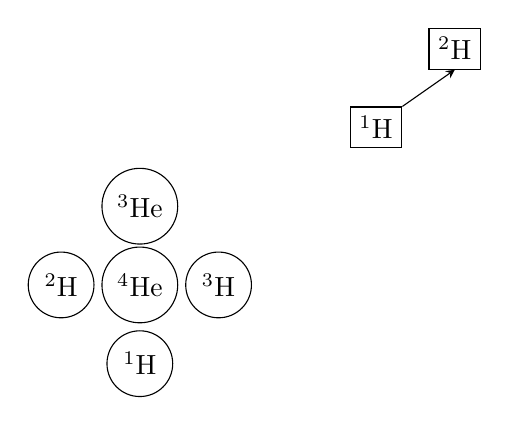
\begin{tikzpicture}
	\path ( 0,2) node [shape=circle,draw] {$\mathrm{{}^{3}He}$}
	( 0,1) node [shape=circle,draw] {$\mathrm{{}^{4}He}$}
	( 0,0) node [shape=circle,draw] {$\mathrm{{}^{1}H}$}
	( 1,1) node [shape=circle,draw, swap] {$\mathrm{{}^{3}H}$}
	
	(-1,1) node [shape=circle,draw] {$\mathrm{{}^{2}H}$};
	
%	\draw (3.7, 3) arc [
%		start angle =60,
%		end angle = 300, 
%		radius = 20pt,
%		color = blue
%	];
	
	%draw [color=blue] (3, 3) circle [radius = 20pt];
	%\draw (4, 3) circle [radius = 20pt];
	
	%(4, 4) node {$\mathrm{{}^{2}H}$};
	
	\node[draw, rectangle] (2H) at (4, 4) {$\mathrm{{}^{2}H}$};
	\node[draw, rectangle]  (1H) at (3, 3) {$\mathrm{{}^{1}H}$};
	
	\draw[-stealth] (1H.north east) -- (2H.south);
	
	%\draw (4, 4) node (A) {$A$} -- (5,5) node (B) {$B$};
	
\end{tikzpicture}
\end{center}


\subsection{Classification of reactions} \label{sub:classificationReactions}

The relevant reactions for the document are:
\begin{equation} \label{eq:nuclearReaction_general}
	0 + 1 \rightarrow 2 + 3
\end{equation}

\begin{equation} \label{eq:nuclearReaction_gammaCapture}
	\gamma + 3 \rightarrow 0 + 1
\end{equation}

Expand  on how the fusion reactions occurs, their conditions and types as well as the differentiation factors with respect to fission processes.

\subsubsection{Capture reactions} \label{ssub:captureReactions}

Also, radiative capture processes are considered at astrophysical energies. Various models could be used for determining potentials. There are clusters and potential models.

\begin{equation}  \label{eq:nuclearReaction_capture}
	X + c \rightarrow  \gamma + X'.
\end{equation}

When $c$ is a proton, the reaction is called radiative proton capture. \cite{brune_davids_2015}

\subsubsection{Exchange reactions}  \label{ssub:exchangeReactions}

\begin{equation}  \label{eq:nuclearReaction_exchange}
	X +  x_1 \rightarrow x_2 + X'
\end{equation}

A development on the $\mathrm{(p,n)}$ reaction kind is given by \cite{whitehead_poxon-pearson_nunes_potel_2022} and for the $\mathrm{(n,p)}$ in \cite{sharma_gandhi_kumar_2022}. \\



\subsubsection{Fusion reactions} \label{ssub:fusionReactions}

\begin{equation}  \label{eq:nuclearReaction_fusion}
	X + X \rightarrow a + X'.
\end{equation}

\subsection{Cross sections} \label{sub:crossSections}

Cross section of a process. 
Partial and total cross sections depending on the reaction type.
Cross sections have relations with the $S$-matrix.

\subsection{Reaction rates} \label{sub:reactionRates}

The ratio that determines the quantity of a nucleus.
\begin{equation}  \label{eq:reactionRate_definition}
	r = A \int_0^{\infty} { E \sigma(E) \exp\left({-\frac{E}{kT}}\right)  dE}.
\end{equation}

\begin{equation} \label{eq:maxwellBoltzmann}
	P(v)dv \propto v^2 \exp{\left({\frac{mv^2}{2kT}}\right)}dv.
\end{equation}

On specifying the rates, it is needed to be considered.

Reaction rates are considered from calculation of transmitted, incident and interacting 
- Reaction rate depends on the density of particles, the velocity and the cross section
-	It is averaged by a convenient distribution. (Maxwell-Boltzman for fermions, Bose Einstein (Planck) for photons)
-	With the rates, abundance evolution is determined 

There are broad classification of reactions. 

\section{The Astrophysical S-factor} \label{sec:sFactor}
\subsection{Motivation and definition} \label{sub:sfactorMotivationDefinition}

There are S factors associated with the energy and they are the path to determine the nature of the potential, which is not necessarily a Yukawa potential.

\begin{equation} \label{eq:sfactor_definition}
	S(E) = E \exp({2\pi\eta}) \sigma({E}).
\end{equation} % ISBN 978-0-521-85635-5.

It is directly proportional to the microscopic cross section of the process $\sigma(E)$ and it represents the rate of a certain nuclear reaction. 
In particular, the astrophysical S-factor 	scales the cross section with a factor proportional to the Coloumb repulsion. 

The $\nu$ factor is defined as 

\begin{equation} \label{eq:sfactor_sommerfeld}
	\eta = \frac{Z_1Z_2e^2}{4\pi\epsilon_0\hbar v}
\end{equation}

where $v$ corresponds to the relative speed between the reactants. \\ 
There is a strong relation of the astrophysical $S$ factor with the center of mass energy. 

Usually this relation depends on the square of the energy of the center of mass $E_{\mathrm{cm}}$. \\

There are topics that are relevant in the frontiers of nuclear astrophysics  \cite{bertulani_kajino_2016}. 

\subsection{General applications} \label{sub:sfactorApplications}

Cross section extrapolation to low energies

Reaction rates and element abundance estimations. 

\chapter{Reactions of astrophysical interest}  \label{ch:reactionsInterest}

Nuclear reactions are part of the core of nuclear astrophysics. They are accountable for the mechanism of production of elements in several astrophysical environments where thermonuclear reactions occur. In particular, there are specially relevant reactions for the explanation of the abundance of elements. For example, some of these reactions are part of critical fusion chains of stars, have challenging extrapolation techniques to low energies, or  exhibit exotic underling physical phenomena.   In this section, a relevant selection of reactions types of will be reviewed. \\

Several reaction kinds and models are given in \cite{descouvemont_2020}.

Screening effect present in light weight nuclear reactions \cite{raiola_migliardi_gyurky_aliotta_formicola_bonetti_broggini_campajola_corvisiero_costantini_et_2002} and a review of screening effect \cite{assenbaum_langanke_rolfs_1987}.

\section{Big bang nucleosynthesis} \label{sec:BBN}

Primordial reactions that where expected to happen after the big bang occurred. For example:

\begin{equation} \label{eq:reaction_2Hpradiative}
	\mathrm{{}^{2}H + p \rightarrow \gamma + {}^{3}H}.
\end{equation}

\section{Stellar fusion}  \label{sec:StellarFusion}

The classical treatment of fusion in stars is given by the classical \cite{burbidge_burbidge_fowler_hoyle_1957}.

Introduce the needed conditions for the creation of stars in the primordial nebula.
Describe how the hydrogen is burnt in the star's core and the associated products. 

\begin{equation} \label{eq:reaction_ppMain}
	p + p \rightarrow d + e^{+} + \nu_e.
\end{equation}

Consider the mechanisms for exchanging heat via radiation and convection.

Explain the required conditions that permits nuclear fusion in the star's nucleus.

\subsection{Light heavy nuclei reactions} \label{sub:lightReactions}

This reaction is governed by the weak force, due to conversion of a proton into a neutron, and by the strong and electromagnetic force.

When it comes to deuterium fusion, this channel is the most abundant.\\

\begin{equation} \label{eq:reaction_2Hdn3He}
	d + d  \rightarrow n + {}^{3}\mathrm{He}.
\end{equation}

The reaction rates of nuclear fusion processes depend on the interaction cross section and the abundance of the reactant nuclei.

\begin{equation}  \label{eq:reaction_2Hdpt}
	d + d \rightarrow p + t.
\end{equation}

The interactions of the previous processes are the electromagnetic and strong force.

\begin{equation} \label{eq:reaction_3HepChain}
	{}^{3}\mathrm{He} + p \rightarrow {}^{4}\mathrm{Li} + \gamma \rightarrow {}^{4}\mathrm{He} + e^{+} +  \nu_e + \gamma.
\end{equation}

This process is unlikely because of the instability of  ${}^{4}\mathrm{Li}$, which decay to ${}^{3}\mathrm{He}$.


\begin{equation} \label{eq:reaction_3Hep3He}
	{}^{3}\mathrm{He} +  {}^{3}\mathrm{He}  \rightarrow {}^{4}\mathrm{He} + 2p.
\end{equation}

This process in known as the pp1 chain.

Exemplify how the reaction mechanisms permits the stability of a star as well as produces He. \\

\subsection{CNO cycle}  \label{sub:CNOCycle}

The carbon burning produces the neutrons that are going to be used in heavy nuclei production. 
The neon burning stats by fusion Neon nuclei with 4He nuclei to produce heavier elements.
The oxygen burning starts are very high temperatures and pressures than the neon and carbon burning due to the high stability of oxygen nuclei. In fact, oxygen nucleus is double magic. \\

When the star has capacity for producing elements like carbon, oxygen and nitrogen,  CNO cycle process can be produced. In particular, reactions take the form 

\begin{equation} \label{eq:reaction_CNO_C}
	\mathrm{{}_{6}^{12}C  \rightarrow {}^{13}_{7}N  \rightarrow {}^{13}_{6}C  \rightarrow {}^{14}_{7}N  \rightarrow {}^{15}_{8}O  \rightarrow {}^{15}_{7}N \rightarrow {}^{12}_{6}C  }.
\end{equation}

\tdplotsetmaincoords{80}{155}
\usetikzlibrary {arrows.meta,bending,positioning} 
\begin{center}
	\begin{tikzpicture}[scale = 5, tdplot_main_coords]		
	
		\draw[-{stealth[scale=2]}, blue] (0, 1) -- (1, 0);
		
		\draw[-{stealth[scale=2]}] (1, 0) -- (0.5, -1);
		
		
		\draw[-{stealth[scale=2]}]  (0.5, -1) -- (-0.5, -1);
		
		\draw[-{stealth[scale=2]}] (-0.5, -1) -- (-1, 0);
		
		\draw[-{stealth[scale=2]}] (-1, 0) -- (0, 1);
	
		
	\end{tikzpicture}
\end{center}


There are other CNO cycles that involve oxygen and fluorine reactions. For instance, the second CNO cycle consists of the following reactions

\begin{equation} \label{eq:reaction_CNO_N}
	\mathrm{{}_{7}^{15}N  \rightarrow {}^{16}_{8}O  \rightarrow {}^{17}_{9}F  \rightarrow {}^{17}_{8}O  \rightarrow {}^{14}_{7}N  \rightarrow {}^{15}_{8}O \rightarrow {}^{15}_{7}N  }.
\end{equation}

There is even a CNO III cycle, which is far more uncommon. 
brig
This branch is less dominant than the first branch.

\subsection{Medium heavy nuclei reactions} \label{sub:mediumHeavyReactions}

These reactions concern nuclei with $A < 28$. Examples of this kind of reaction include the $\mathrm{{}^{12}C + {}^{12}C}$,  $\mathrm{{}^{12}C + {}^{16}O}$ and the  $\mathrm{{}^{16}O + {}^{16}O}$ fusion reactions. Most of these reactions result in different channels. \\ 

With respect to the carbon fusion reaction, the principal channel is given by: 

\begin{equation} \label{eq:reaction_C12fusion_alpha20Ne}
	\mathrm{{}^{12}C + {}^{12}C \rightarrow {}^{4}He + {}^{20}Ne}. 
\end{equation}

On the other hand, the main channel of the oxygen fusion reaction occurs in the following manner:

\begin{equation} \label{eq:reaction_O12fusion_alpha28Si}
	\mathrm{{}^{16}O + {}^{16}O \rightarrow {}^{4}He + {}^{28}Si}. 
\end{equation}

Additionally, there are inelastic channels associated with $\mathrm{{}^{16}O}$ which could increase the probability of occurrence for the overall reactions.  \\

\begin{center}
	\begin{tikzpicture}

		\node (center) at (0, 0) {$\mathrm{{}^{16}O + {}^{16}O}$};
		
		%\node (CH1) at (6, 3) {$\mathrm{{}^{4}He + {}^{28}Si}$};
		%\node (CH2) at (3, 3) {$\mathrm{p + {}^{31}P}$};
		%\node (CH3) at (0, 3) {$\mathrm{d + {}^{30}P}$};
		%\node (CH4) at (-3, 3) {$\mathrm{\alpha \alpha + {}^{30}P}$};
		%\node (CH5) at (-6, 3) {$\mathrm{n + {}^{31}{S}}$ };
		
		\node (CH1) at (3, 6) {$\mathrm{\alpha + {}^{28}Si}$};
		\node (CH2) at (3, 3) {$\mathrm{p + {}^{31}P}$};
		\node (CH3) at (3, 0) {$\mathrm{d + {}^{30}P}$};
		\node (CH4) at (3, -3) {$\mathrm{\alpha \alpha + {}^{30}P}$};
		\node (CH5) at (3, -6) {$\mathrm{n + {}^{31}{S}}$ };
		
		\draw[-stealth] (center) -- (CH1);
		\draw[-stealth] (center) -- (CH2);
		\draw[-stealth] (center) -- (CH3);
		\draw[-stealth] (center) -- (CH4);
		\draw[-stealth] (center) -- (CH5);
		
		\node (center2) at (10, 0) {$\mathrm{{}^{12}C + {}^{12}C}$};
		
		\node (CH6) at (13, 6) {$\mathrm{\alpha + {}^{20}Ne}$};
		\node (CH7) at (13, 3) {$\mathrm{p + {}^{23}Na}$};
		\node (CH8) at (13, 0) {$\mathrm{d + {}^{22}Na}$};
		\node (CH9) at (13, -3) {$\mathrm{\alpha \alpha + {}^{16}O}$};
		\node (CH10) at (13, -6) {$\mathrm{n + {}^{23}{Mg}}$ };
		
		\draw[-stealth] (center2) -- (CH6);
		\draw[-stealth] (center2) -- (CH7);
		\draw[-stealth] (center2) -- (CH8);
		\draw[-stealth] (center2) -- (CH9);
		\draw[-stealth] (center2) -- (CH10);
		
	\end{tikzpicture}
\end{center}


There are more cycles of capture reaction. An example regarding the MgAl cycle is given in \cite{lotay_doherty_janssens_seweryniak_albers_almaraz-calderon_carpenter_champagne_chiara_hoffman_et_2022}.

Explain the different chains going on during the carbon-oxygen combustion to heavier elements like iron or silicon.

The Trojan horse method\cite{spitaleri_mukhamedzhanov_blokhintsev_cognata_pizzone_tumino_2011}

nucleosynthesis in massive stars \cite{pignatari_hirschi_wiescher_gallino_bennett_beard_fryer_herwig_rockefeller_timmes_et_2012}

12C + 12C Wave packet dynamics\cite{diaz-torres_wiescher_2018}
nonresonant Bayersian \cite{li_fang_bucher_li_ru_tang_2020}
Modified sfactor \cite{luo_wen_lin_yang_jia_yang_huang_chang_zhang_yang_et_2022}
Trojan horse \cite{mukhamedzhanov_pang_kadyrov_2019}
\cite{mukhamedzanov_2022}
full-microscopical \cite{taniguchi_kimura_2021}
multichannel folding \cite{assuncao_descouvemont_2016}
screening effects \cite{koyuncu_soylu_2018}

correlation between carbon fusion reactions \cite{notani_esbensen_fang_bucher_davies_jiang_lamm_lin_ma_martin_et_2012}
constraint 12C + 12C based on 12C + 13C reaction \cite{zhang_wang_tudor_bucher_burducea_chen_chen_chesneanu_chilug_gasques_et_2020}

16O + 16O cross sections \cite{duarte_gasques_oliveira_zagatto_chamon_medina_added_seale_alcantara-nunez_rossi_et_2015}
\cite{kuronen_keinonen_tikkanen_1987}

oxygen isotopes fusion \cite{thomas_chen_hinds_meredith_olson_1986}
coupled channels \cite{guimin_deji_xiaowu_1992}

12C + 16O semi-microscopic cluster \cite{ferreira_lubian_linares_ermamatov_yepez-martinez_hess_2019}
low-energy resonances \cite{torilov_maltsev_zherebchevsky_2021}
12C + 16O based on yields of 12C + 16O and 12C + 18O \cite{chan_bohn_vandenbosch_sielemann_cramer_bernhardt_bhang_chiang_1979}

selected oxygen-oxygen and oxygen-carbon reactions \cite{kovar_geesaman_braid_eisen_henning_ophel_paul_rehm_sanders_sperr_et_1979}
\cite{wang_ren_bai_2020}
12C + 12C and 16O + 16O \cite{assuncao_descouvemont_2015}

12C and 24 Mg resonances \cite{descouvemont_2021}
Fusion hidrance 12C + 24Mg \cite{montagnoli_stefanini_jiang_colucci_goasduff_brugnara_mazzocco_siciliano_scarlassara_corradi_et_2020}

heavy-ion  reactions \cite{nobre_chamon_gasques_carlson_thompson_2007}


\section{Supernovae and other explosive environments} \label{sec:explosive}

Additional fusion reactions with nuclei with $A > 28$ are present at the last stages of the life of a star. There are two main environments: The stellar fusion and explosive events fusion.


\subsection{Heavy nuclei reactions} \label{sub:heavyReactions}

There is a silicon burning process with the following description 

\begin{equation} \label{eq:reaction_28Sialpha}
	\mathrm{{}^{28}_{14}Si +{}^{4}_{2}He \rightarrow {}^{32}_{16}S}.
\end{equation}

Silicon burning is another process.\\

\begin{equation} \label{eq:reaction_28Sifusion_alpha56Fe}
	\mathrm{{}^{28}Si + {}^{28}Si \rightarrow {}^{4}He + {}^{56}Fe }.
\end{equation}

This reaction is essential since the $\mathrm{{}^{56}Fe}$ nucleus has the maximum binding energy. Then, fusion reactions of heavier nuclei tend to be less spontaneous.Then,  this chain of reactions continues until the process in there 56-Ni is reached.

\begin{equation}  \label{eq:reaction_52Fealpha}
	\mathrm{{}^{52}_{26}Fe +{}^{4}_{2}He \rightarrow {}^{56}_{28}Ni}.
\end{equation}


\subsection{The s and p processes} \label{sub:spProcesses}

There exists the s and  the r processes. Each permits to form heavier nuclear elements products. Now, there are aspects of the particularities of the production of the nuclei that  are currently  unknown \\

On the other hand, protons are captured at the ending of the life of a gigantic star. This process, which occurs at high densities and temperatures, is referred as proton capture. In particular, under astrophysical scenarios like supernovas, the rapid proton capture, in addition to the neutron capture,  produces a considerable amount of the heavy nuclei. This process is referred as rapid proton capture, or rp process. \\ 

Further processes are not viable because they are not exothermic and potential heavier nuclei than 56-Ni are photodisintegrated. At this scale of energy, nuclear reactions start to behave similarly than chemical equilibrium reactions. 

The conditions are associated with the mass. Particularly, depending on the mass regime, star evolution can differentiate. For instance, there are brown dwarfs, sun like stars. \\

There is an evolution process that is ruled by different instances. Each instance can be regarded as a region in the Hertzsprung-Russell diagram. This diagram consists of a two dimensional scatter plot of the intensity with respect to the spectral type of a star. Particularly, there are regions associated to the different instances of the life of a star: Main sequence (Hydrogen burning stars), red stars, neutron stars, supernova of kinds Ia Ib and other instances. \\

Electron degeneracy prevents the white dwarf to collapse and the neutron degeneracy pressure prevents the neutron star to collapse. These limits account for relativistic Fermi gas and neutron degeneracy with a model from general relativity. \\

Indicate that there exists different channels of production depending on the existence of neutron capture or fission products. Additionally, explain the needed conditions in order to those processes to occur. \\ 

If mass increases further, there is no place to any degeneracy compensation so the star would collapse to a black hole.

\section{Active research topics} \label{sec:activeResearch}

Enumerate the broad ranges of phenomena that are left to be explained.  \\

Introduce current approaches of some of the unsolved questions on nuclear astrophysics, particularly on the last instances of fusion in the star's lifetime. \\

There are various types of  supernovae. However, there are mechanisms that are not considered and yet not well explained. \\

Current experiments in detection of heavy nuclei are essential to determine the distribution of elements, specially in events like the fusion of neutron stars.\\ 

Review on active research topics and current challenges in nuclear astrophysics in general \cite{arcones_bardayan_beers_bernstein_blackmon_messer_brown_brown_brune_champagne_et_2017} and on low-energy nuclear physics \cite{carlson_carpenter_casten_elster_fallon_gade_gross_hagen_hayes_higinbotham_et_2017} are given.



\chapter{Astrophysical S-factor models} \label{ch:sfactorModels}

There are several methods for estimating the astrophysical S-factor. Each method is more convenient depending on the nature of the reaction. For example, method accuracy can vary depending on  the reaction type or the existence of resonant phenomena. Additionally, the methods are based on a specific approach when modeling the S-factors. In this section, the principal methods of estimating the astrophysical S-factors will be reviewed.

\section{Microscopic models} \label{sec:microscopicalModels}

Microscopic models are based on first principles and usually require assumptions about the nucleus and its structure. \\ 

\begin{equation} \label{eq:micro_hamiltonian}
	H = \sum_{k} T_k + \sum_{k} V_k (r) + \sum_{k \neq j} V_{kj}(r).
\end{equation}

On the other, clusters consider the system of interactant nuclei as a whole. In particular, there are models based on \textit{ab initio} assumptions about a particular set of nuclei.  \\

$NN$ and $NNN$ interactions.

\begin{center}
	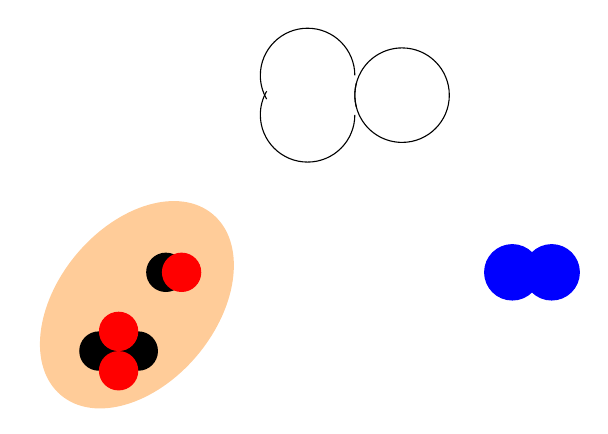
\begin{tikzpicture}		
		\fill[orange, fill opacity=0.4] (0.6,0.2)[rotate = 50] ellipse (1.5 and 1.0);
		
		\fill[black] (0.25, 0) circle (0.25);
		\fill[black] (-0.25, 0) circle (0.25);
		\fill[red] (0, 0.25) circle (0.25);
		\fill[red] (0, -0.25) circle (0.25);
		
			
		\fill[black] (0.6, 1.0) circle (0.25);
		\fill[red] (0.8, 1.0) circle (0.25);
		
		
		%\filldraw [blue] (2,2) -- (2,3) -- (3, 3) -- (3, 2) -- (2,2);
			
		\draw (3,3) arc (0:-210:0.6);
		\draw (3,3.5) arc (0:210:0.6);
		
		\draw (4.2,3.25) arc (0:-195:0.6);
		\draw (4.2,3.25) arc (0:195:0.6);
		
		
		\filldraw[blue] (5, 1) circle (10pt);
		\filldraw[blue] (5.5, 1) circle (10pt);
		
		
		%\draw (4, 4.5) arc(0:-300:0.6)  ;
		
		%\filldraw [green] (3, 3) circle (0.05) ;
		%\filldraw [blue] (4, 4.5) circle (0.05) ;
		
	\end{tikzpicture}
\end{center}


The \textit{ab initio} no core shell model is presented in \cite{barrett_navratil_vary_2013}. \\

A more detailed survey on cluster models \cite{beck_2012}.

\begin{equation}  \label{eq:micro_folding}
	\int \int \rho(r_1) \rho(r_2) dr_1 dr_2. 
\end{equation}

The mass and nuclear density of the nuclei can be modeled as:

\begin{equation} \label{eq:micro_density}
	\rho(r) = \frac{\rho_0}{1 + \exp{\left(\frac{r - R}{a}\right)}}.
\end{equation} 

Non-local calculations. Multi-body calculations. \\

Also, nuclei deformation can be considered in models. For example, there are models with no-core shell. \\

More sophisticated models use effective field theory for calculations. The general principle of these theories is the low-energy approximate solution of the physics described in quantum chromodynamics. \\

\begin{equation} \label{eq:micro_lagrangian_nucleons}
	\mathcal{L} = N^{\dagger}i\hbar\gamma^\mu\partial_\mu N + ... .
\end{equation}

Diagrams associated with the processes of low-energy nuclear force. Mediators are mesons like pions. \\

Modern theories \cite{marcucci_nollett_schiavilla_wiringa_2006}

Three body \cite{grigorenko_danilin_efros_shulgina_zhukov_1998}

Ab initio \cite{neff_feldmeier_langanke_2011}
\cite{navratil_quaglioni_hupin_romero-redondo_calci_2016}
\cite{navratil_bertulani_caurier_2006}
\cite{atkinson_navratil_hupin_kravvaris_quaglioni_2022}
tensor force \cite{arai_aoyama_suzuki_descouvemont_baye_2013}

No core shell model \cite{dohet-eraly_navratil_quaglioni_horiuchi_hupin_raimondi_2016}

Shell model \cite{dong_wang_michel_ploszajczak_2022}
\cite{tazawa_1974}

Effective field theory \cite{sadeghi_khalili_godarzi_2013}
\cite{higa_premarathna_rupak_2022}

Multicluster \cite{dufour_descouvemont_1997}
\cite{simenel_keser_umar_oberacker_2013}

Hauser-Feshbach \cite{jayatissa_avila_rehm_talwar_mohr_auranen_chen_gorelov_hoffman_jiang_et_2022}

Break up effects \cite{shubhchintak_descouvemont_2022}

Linear chain \cite{baba_taniguchi_kimura_2022}

Hartree-Fock \cite{leanh_minhloc_2022}


\section{Matrix models}  \label{sec:matrixModels}

The matrix models permit the modeling of resonances with an appropiate fitting of free parameters. In particular, the main formalism in this approach is the R-matrix model. \cite{lane_thomas_1958}.

\begin{equation}  \label{eq:rmatrix_elements}
	R_{cc'} = \sum_k {\frac{\gamma_{ck} \gamma_{c'k}}{E - E_k}}.
\end{equation}

The sum is over levels and the elements are parameterized as channels. 


\begin{equation} \label{eq:rmatrix_sfactor}
	S(E) = S_r \frac{\Gamma^2/4}{(E-E_r + \Delta)^2 + (\Gamma/2)^2}.
\end{equation}

There is parameter $P(E)$ which is expressed as: 

\begin{equation} \label{eq:rmatrix_penetrationFactor}
	P= \frac{\Gamma}{F_l^2 + G_l^2},
\end{equation}

where the functions $F_l = F_l(ka)$ and $G_l = G_l(ka)$ are the Coulomb functions evaluated at a particular $\rho = ka$. In addition, another parameter $Q$ is given: 

\begin{equation} \label{eq:rmatrix_QFactor}
	Q = \frac{\Gamma}{F_lG_l' + G_lF_l'}.
\end{equation}

On the other hand, the phase shift is given by:

\begin{equation}  \label{eq:rmatrix_phaseShift}
	\delta = \delta_{\mathrm{HS}} + \delta_R.
\end{equation}

The model includes free parameter $a$ which is called the radius channel. \\

Resonances arrives from poles. A description on the physical consideration of poles in the scattering (S-matrix) is given in \cite{ramirezjimenez_kelkar_2018}.


In primordial nucleosynthesis \cite{desouza_iliadis_coc_2019} big-bang 3He and several reactions \cite{sparta_pizzone_bertulani_hou_lamia_tumino_2020}. \\

Bayesian fitting methods \cite{odell_brune_phillips_2022}.

Litium detueron capture \cite{grineviciute_lamia_mukhamedzhanov_spitaleri_lacognata_2015}. \\

10B proton non-radiative \cite{kolk_macon_deboer_anderson_boeltzig_brandenburg_brune_chen_clark_danley_et_2022} and similarly \cite{sieverding_randhawa_zetterberg_deboer_ahn_mancino_martinez-pinedo_hix_2022}. 10B radiative and resonances in 11C inverse kinematics \cite{kaur_guimaraes_zamora_assuncao_alcantara-nunez_delara_zevallos_ribeiro_lichtenthaler_pires_et_2022}.

Alpha capture reactions of carbon \cite{schurmann_gialanella_kunz_strieder_2012}.  Hybrid potential/R-matrix \cite{sparenberg_2005}. \\ 13C alpha capture and 16O determination \cite{prusachenko_bobrovsky_bondarenko_bokhovko_gurbich_ketlerov_2022}.

Proton capture carbon \cite{burtebaev_igamov_peterson_yarmukhamedov_zazulin_2008} for C12 and \cite{chakraborty_deboer_mukherjee_roy_2015} for C13 and \cite{genard_descouvemont_terwagne_2010} for the same reaction . \\

15N capture in \cite{barker_2008} and 14N in \cite{angulo_champagne_trautvetter_2005}. also on 14N proton capture \cite{formicola_imbriani_costantini_angulo_bemmerer_bonetti_broggini_corvisiero_cruz_descouvemont_et_2004}.

There is also the K-matrix model as an alternative of the R-matrix model \cite{humblet_1990}.

Alternative formulation of R-matrix \cite{brune_2002}.


\section{Potential models} \label{sec:potentialModels}

The electromagnetic potential can be modeled as an uniform charged sphere potential. 

\begin{equation} \label{eq:potential_EM}
	V_{\mathrm{EM}} = 	\left\{\begin{array}{l}
		\begin{split}
			\frac{Z_1Z_2e^2}{4\pi\epsilon_0R}\left(\frac{3}{2} - \frac{r^2}{2R^2}\right), \quad &r \le R \\ 
			\frac{Z_1Z_2e^2}{4\pi\epsilon_0r}, \quad &r > R	
		\end{split}
	\end{array}\right.
\end{equation}

In addition, in order to account for the nuclear force, there are several potentials. For instance, in a first approximation, there is the step potential.
\begin{equation} \label{eq:potential_squareWell}
	V_{\mathrm{SqW}} = -V_0\theta(r).
\end{equation}

Yakovlev et. al model \cite{yakovlev_beard_gasques_wiescher_2010} consists of an estimation of the potential that is similar to the parabolic potentials with free parameters that attempt to account for the effects of the nuclear and electromagnetic interactions.  \\


\begin{equation} \label{eq:potential_Yakovlev}
	V_{\mathrm{YAK}} = 	\left\{\begin{array}{l}
		\begin{split}
			E_c\left(3 - \frac{r^2}{R_c^2}\right), \quad &r \le R_{c1} \\ 
			\frac{Z_1Z_2e^2}{r}, \quad &r > R_{c1}	
		\end{split}
	\end{array}\right.
\end{equation}

Additionally, the model distinguish between classical allowed and forbidden regions.  For the first region, where $E < E_c$, the astrophysical S-factor is estimated as:

\begin{equation}  \label{eq:potential_Yakovlev_sfactor}
	S(E) = S(0)\sqrt{\frac{Ec}{E}} [\exp{(\Psi(E))+ k\xi} ],
\end{equation}

where $\xi$ is a free parameter of the model that accounts for the deviation from free particle behaviour of the S-factor. On the other hand, $S(0)$ corresponds to the zero-energy extrapolation of the S-factor. \\

uses the WKB approximation for estimating the wave function. Then, the astrophysical S-factor is determined by a phenomenological equation. \\


\begin{equation}  \label{eq:potential_Yakovlev_psiWKB}
	\Psi(E) = 2\pi\eta(E) + \Phi(E),
\end{equation}

where $\eta(E)$ is the Sommerfeld parameter, and $\Phi(E)$ is the wavefunction calculated by the WKB. Further details on the calculation of the last parameter are presented in section \ref{sub:tunnelingPhenomena}. \\

In order to the potential to be more realistic, a Woods-Saxon potential consider a smooth behavior.

\begin{equation} \label{eq:potential_WoodsSaxon}
	V_{\mathrm{WS}}(r) = \frac{V_0}{1 + \exp  \left({\frac{r-R}{a}}\right)},
\end{equation}


where $V_0$ represents the potential depth, $a$ the parametrization and $R$ a computed radius which is defined as: 

\begin{equation} \label{eq:potential_WoodsSaxon_radius}
	R = r_0(A_1^{1/3} + A_2^{1/3}).
\end{equation}

On the other hand, it is relevant, specially at low energies, the inclusion of angular momentum effects in the potential. In order to account for that effect, there is the potential with angular moment. \\

Also, spin orbit coupling effect is noticeable for certain kind of reactions. The contribution to the potential associated with this effect is expressed as:

\begin{equation}  \label{eq:potential_spinOrbit}
	V_{\mathrm{SO}}(r) = k\langle L \cdot S \rangle  \frac{1}{m_{\pi}r} \frac{d}{dr} V(r),
\end{equation}

where the coupling  $  \langle L \cdot S \rangle$ is expressed as: 

\begin{equation}  \label{eq:potential_spinOrbit_LSexpansion}
	\langle L \cdot S \rangle = J(J+1) - l(l+1) - s(l+1).
\end{equation}

In the radiative capture reactions, cross sections are computed based on electromagnetic field operators. In particular 

\begin{equation}  \label{eq:radiativeCapture_operator}
	\sigma_m = \sum_{k}{\langle k | \mathcal{O} | m \rangle} C_{klm}.		
\end{equation}


Double exponential potentials: 

\begin{equation} \label{eq:potential_doubleExponential}
	V_{\mathrm{DE}}(r) = - V_0 \left(e^{\alpha_1 r} + e^{\alpha_2 r} \right)^{-1}.
\end{equation}

Cluster potential:

\begin{equation} \label{eq:potential_cluster}
	V_{\mathrm{CL}}(r) = - V_0 \exp{(-\alpha r^2 )} + V_1 \exp{(\beta r)}.
\end{equation}

Gaussian exponential: 

\begin{equation} \label{eq:potential_gaussianExponential}
	V_{\mathrm{GE}}(r) = - V_0 \exp{(-\alpha r^2 )}.
\end{equation}

Yukawa potential  which includes screening effect.

\begin{equation} \label{eq:potential_Yukawa}
	V_{\mathrm{Y}} = -\frac{c}{4\pi\epsilon_0}e^{-\mu r}.
\end{equation}

And, potentials with non-locality are also found in literature. For example, there is the São Pablo potential that accounts for the effect of non-local interactions between the interactant nuclei. \\

Capture reaction review light nuclei\cite{ghasemi_sadeghi_2018}
\cite{dubovichenko_dzhazairov-kakhramanov_2012}

7Be radiative capture \cite{tursunov_turakulov_kadyrov_blokhintsev_2021}
\cite{bertulani_1996}

9Be radiative capture \cite{kabir_nabi_2021}

p2H radiative capture \cite{dubovichenko_dzhazairov-kakhramanov_2009}

2Hdp reaction \cite{czerski_huke_heide_ruprecht_2006}

13C radiative capture \cite{kabir_irgaziev_nabi_2020}
\cite{dubovichenko_2012}

11C radiative capture\cite{kabir_irgaziev_nabi_sagheer_2022}

16O fusion \cite{diaz-torres_gasques_wiescher_2007} \\

Sao pablo \cite{chamon_2007}


\begin{equation} \label{eq:potential_SaoPablo}
	V_{\mathrm{SPP}} (r) = V_{\mathrm{F}} (r)e^{-4V^2/c^2}.
\end{equation}


\begin{equation} \label{eq:potential_SaoPablo_speed}
	V^2 = \frac{2}{\mu} \left( E - V_{\mathrm{F}}(r) - V_{\mathrm{C}}(r) \right),
\end{equation}

where the reduced mass is $\mu$, the Coulomb potential is $V_{\mathrm{C}}(r)$ and the folding potential  $V_{\mathrm{F}}(r)$ is expressed as:


\begin{equation} \label{eq:potential_SaoPablo_folding}
	V_{\mathrm{F}}(r) = \int \int \rho_1(\vec r_1)  \rho_2(\vec r_2) \delta(\vec r - \vec r_1 +  \vec r_2) {d\vec{r}_1}  {d\vec{r}_2}.
\end{equation}

\begin{center}
	\begin{tikzpicture}		
	\shade[ball color = black,
	opacity = 0.5
	] (-3,0,0) circle (20pt);
	
	
	\shade[ball color = black,
	opacity = 0.5
	] (3,0,0) circle (20pt);


	\fill[black] (-0.25, 4, 0) circle (2pt) ;
	
	\draw[-{Stealth[scale=2]}] (-3, 0, 0) -- (3, 0, 0);
	
	\draw[-{Stealth[scale=2]}] (-3, 0, 0) -- (-0.25, 4, 0);
	
	\draw[{Stealth[scale=2]}-] (3, 0, 0) -- (-0.25, 4, 0);
		
	\draw (0, -0.25, 0) node {$\vec R$};
	\end{tikzpicture}
\end{center}


Optical model \cite{amer_penionzhkevich_2021}

\begin{equation}  \label{eq:potential_Optical}
	V(r) = V_R(r) + iW_R(r).
\end{equation}

Woods-Saxon \cite{salamon_baran_vertse_2016}
\cite{singh_sukhvinder_kharab_2013A}

\begin{equation} \label{eq:potential_WoodsSaxon2}
	V_{\mathrm{WS}} = -V_0 f(r),
\end{equation}

\begin{equation}  \label{eq:potential_WoodsSaxon2_fermiDirac}
	f(r) = \frac{1}{1 + \exp {\left(\frac{r- R}{a}\right)}}.
\end{equation}

Energy dependent model \cite{singh_sukhvinder_kharab_2013B}

$V_0(E)$

Cross section deduced potential \cite{bass_1977} \cite{nandi_swami_gupta_kumar_chakraborty_manjunatha_2022}




\section{Empirical formulas} \label{sec:empiricalFormulas}

%Explain the forces and interactions going on in a star. Highlight what makes a star stable.

For resonant reactions, the Breit-Wigner formula

\begin{equation} \label{eq:empirical_breitWigner}
	S(E) = S_r \frac{\Gamma^2_r/4}{(E-E_r)^2 + (\Gamma_r/2)^2}.
\end{equation}

And some empirical formulas can be given. 

On the other hand, non-resonant reactions S-factors can be calculated with polynomial interpolations and fits. 

In particular, there is a polynomial expansion that is reported in literature to be useful. 


\begin{equation} \label{eq:empirical_exponential}
	S(E) = \exp{(g_0 + g_1E + g_2E^2 + g_3E^3 + ...)}.
\end{equation}

Also, more generic expansions are modeled by fitting a Laurent series expansion. 

\begin{equation}  \label{eq:empirical_laurent}
	S(E) =\frac{ a_{-1}}{E} + a_0 + a_1 E + a_2 E^2 + ... \ .
\end{equation}

For some reactions, $a_{-1} = 0$, then they are described as a Taylor series expansion.

\begin{equation}  \label{eq:empirical_polynomial}
	S(E) = a_0 + a_1E + a_2 E^2 + ... \ .
\end{equation}


On the other hand, empirical formulas can mix resonant and non-resonant terms. For example, consider the expression: 

\begin{equation}  \label{eq:empirical_hybridPolynomial}
	S(E) =  \sum _{k = 0}^{N} {a_kE^k} + \sum_{l = 1}^{M} {\frac{\Gamma_l^2/4}{(E - E_l)^2 + \Gamma_l^2/4}},
\end{equation}

Analogously, if the non-resonant term has a polynomial form, the S-factor hybrid resonant and non-resonant expansion is expressed as:

\begin{equation}  \label{eq:empirical_hybridExponential}
	S(E) =  \exp { \left( \sum _{k = 0}^{N} {a_kE^k} \right) } + \sum_{l = 1}^{M} {\frac{\Gamma_l^2/4}{(E - E_l)^2 + \Gamma_l^2/4}},
\end{equation}

where $N$ is the maximum order of the polynomial to be fitted, which accounts for the non-resonant behavior of the reaction, and $M$ represents the number resonances present in the reaction. 

Applications in direct capture \cite{jennings_karataglidis_shoppa_1998}.  Exchange reactions $\mathrm{(p, n)}$ kind \cite{hussein_abdullah_2020}.

Charged particle collisions non-resonant \cite{ueda_sargeant_pato_hussein_2002} and resonant \cite{ueda_sargeant_pato_hussein_2004}. \\

Fusion reactions, which is a more sophisticated model \cite{beard_afanasjev_chamon_gasques_wiescher_yakovlev_2010}.

\begin{equation} \label{eq:empirical_yakovlev}
	S(E) = \sum_{k=0}^{N} {a_kE^k} + \left(1 + \exp{\left(1 +  \frac{E - E_c}{D}\right)}\right)^{-1} \sum_{l=0}^{M} {b_lE^l}  .
\end{equation}

\chapter{S-factor calculations for selected reactions} \label{ch:sfactorCalculations}

In this chapter, the S-factor calculation for a selected list of reactions will be presented. The list of reactions distinguish between resonant and non-resonant reactions. Additionally, this list includes reactions from Big Bang nucleosynthesis, pp-chain, CNO cycle and middle heavy nuclei fusion astrophysical environments.  \\




In order to account for the best predictions for the astrophysical S-factors of the referred reactions, a motivation on the selection of a particular model will be mentioned, as well as the calculation consideration used to perform the calculations will be detailed for each reaction. \\


Further details about capture reactions with single-particle states is given by \cite{huang_bertulani_guimaraes_2010}. \\

Additional, about pp-chain is given by \cite{adelberger_garcia_robertson_snover_balantekin_heeger_ramsey-musolf_bemmerer_junghans_bertulani_et_2011}.

Computer libraries that were used:

Python \cite{rossum_drake_2009}, Pandas \cite{mckinney_2010}, NumPy \cite{harris_millman_vanderwalt_gommers_virtanen_cournapeau_wieser_taylor_berg_smith_et_2020}, SciPy \cite{virtanen_gommers_oliphant_haberland_reddy_cournapeau_burovski_peterson_weckesser_bright_et_2020}, Matplotlib \cite{hunter_2007}.


\section{Non-resonant reactions} \label{sec:nonResonant}

The starting point in the process of analysis of reaction is the study of its non-resonant part. \\

Light heavy selected reactions are $\mathrm{{}^{2}{H} (p, \gamma) {}^{3}{He}} $ and $\mathrm{{}^{2}{H}(d,p){}^{3}{H}} $. On the other hand,  $\Cfusion$  and $\Ofusion$ are the fusion reactions to be considered. \\

Empirical formulas are initially considered for the light heavy S-factor description. In particular, the non-resonant part of the equations \ref{eq:empirical_hybridExponential}  and \ref{eq:empirical_hybridPolynomial} are fitted to experimental data.  \\

In addition, a correction factor that accounts for the electron screening effect observed at low-energies  in the $\mathrm{{}^{2}H(d, p){}^{3}H}$ reaction is included. \\
 
On the other hand, fusion reactions are described by the Yakovlev et. al empirical formula \cite{beard_afanasjev_chamon_gasques_wiescher_yakovlev_2010} and potential model  \cite{yakovlev_beard_gasques_wiescher_2010}. 

Microscopical and matrix model approaches are  used to be describe all the selected reactions.



%For me, writing represents discipline and creativity. And, this is a great chance to convert our ideas into products. 
%Even though some times writing was seen as an undesirable activity, specially at moments when there were deadlines or when it was asked to write about unrelated things in your life, I genuinely hope that we have found a path towards more enjoyable writing. 

% Being tested was, at some moment, my hardest pressure. I think that most of the times there was a need of making sure that everything was according to the required standards imposed by others. Then, writing was seen as a passive exercise that would happen to be useful for activities. Now, I propose that we might think writing as an active and creative exercise. To think in writing as the ultimate act of projecting your ideas as well as the deserved result of this significant project. So, this shift in the purpose of writing truly represents a step ahead for increasing our independence and for fostering our career goals.
 
 %Then, those standards that were once imposed, by what it seemed to be the external and restrictive interest of others, are converted in friendly procedures that you truly need. It is now the time to you to create the standards, which would be rather called, the guidelines and opportunities for your creations. 
 
 
\subsection{Calculation considerations} \label{sub:considerationsNonResonant}

Empirical formulas were determined by fitting parameters to best describe experimental data. In particular, the parameters chosen minimized the chi-squared $\chi^2$ function as it is described in appendix \ref{ap:fitting}. In some cases, it was necessary to constraint the interval of validity of the parameters in order to avoid unphysical behaviour of the fittings. Further details about this constraints can be found in section \ref{sec:empiricalFitting}. \\

For the case of Yakovlev et. al potential model, an analytical calculation was performed. In this calculation, the parameters given in \cite{yakovlev_beard_gasques_wiescher_2010} were used for the selected fusion reactions.  \\

In the Yakovlev model, there is a fitting of the parameters in the following way.  The free parameters are $\delta$, $E_c$ and $\xi$. In particular, $E_c$ can be determined by the following expression:

\begin{equation} \label{eq:potential_Yakovlev_Ec}
	E_c = \frac{\alpha}{R},
\end{equation}

where $\alpha = \sqrt{Z_1Z_2e^2}$ and $R$ is a parameter that is determined as:

\begin{equation} \label{eq:potential_Yakovlev_R}
	R = R_0 + \Delta R_{1} |2Z_1 - A_1| + \Delta R_{2}|2Z_2 - A_2|.
\end{equation}

In particular, the parameter $R_0$ depends on the reactant nuclei while the parameters $\Delta R_{1}$ and $\Delta R_{2}$ can assume two values per pair of reactant nuclei. For instance, the values are given in the following way: 

\begin{equation} \label{eq:potential_Yakovlev_R1}
	\Delta R_1= 	\left\{\begin{array}{l}
		\begin{split}
			\Delta R_{10}, \quad & 2Z_1 > A_1\\ 
			\Delta R_{11}, \quad & 2Z_1 < A_1
		\end{split}
	\end{array}\right.
\end{equation}

Analogously, $\Delta R_2$ is determined as: 

\begin{equation} \label{eq:potential_Yakovlev_R2}
	\Delta R_2= 	\left\{\begin{array}{l}
		\begin{split}
			\Delta R_{20}, \quad & 2Z_2 > A_2\\ 
			\Delta R_{21}, \quad & 2Z_2 < A_2
		\end{split}
	\end{array}\right.
\end{equation}

The numerical values that were provided in \cite{yakovlev_beard_gasques_wiescher_2010} for each of the reactions to be studied are contained in section \ref{sec:fittingParams}. \\

Although Yakovlev et. al model is used for middle-heavy fusion reactions, is not expected to work for radiative capture reactions since it predicts a decrement of the S-factor for all energies. In contrast, the S-factor increases in radiative capture reactions.  \\


\subsection{Results and analysis} \label{sub:resultsAnalysisNonResonant}

\graphWrapper{
	\subGraph{2H(d,p)3H-poly12345}{Polynomial fits.}
	\subGraph{2H(d,p)3H-exp12345}{Exponential fits.}
	\subGraph{2H(d,p)3H-exp5-poly5-best}{Best fits.}[1]
}
{2H(d,p)3H}{Polynomial and exponential fits $\ddexchange$ reaction}{Empirical formulas fitted to the S-factor for the  $\ddexchange$ reaction. In panel a), poly1, poly2, poly3, poly4, and poly5 represent fits to polynomials function from first order up to fifth order respectively.  Similarly, in panel b), exp1, exp2, exp3, exp4 and exp5 represent the exponential fit up to fifth order. Additionally, in panel c) the poly5-exclude graph corresponds to a poly5 like fit without data from RA02 and GR95. The black points are related with experimental data which was taken form different sources.}

%\graph{2H(d,p)3H}{D deuterium capture}{Detailed caption reaction}

At low-energies as far as $ \mathrm{10^{-3} \ MeV}  <  E<\mathrm{10^{-2} \ MeV}$, an exponential-like damping of the S-factor is observed. In fact, this  behavior could explained due to the electron screening effect \cite{raiola_migliardi_gyurky_aliotta_formicola_bonetti_broggini_campajola_corvisiero_costantini_et_2002}.


GR85 \cite{greife_gorris_junker_rolfs_zahnow_1995}
KR87a \cite{krauss_becker_trautvetter_rolfs_brand_1987}
LE06a \cite{leonard_karwowski_brune_fisher_ludwig_2006}
RA02 \cite{raiola_migliardi_gyurky_aliotta_formicola_bonetti_broggini_campajola_corvisiero_costantini_et_2002}
SC72 \cite{schulte_cosack_obst_weil_1972}
TU11 \cite{tumino_spitaleri_mukhamedzhanov_typel_aliotta_burjan_delsanto_kiss_kroha_hons_et_2011}

\graph{2H(d,p)3H-screening-exp5-poly5-exclude}{Screening effect $\ddexchange$ reaction}{Polynomial fits to the experimental data with the consideration of the screening effect. The curve fit labeled as \textit{screening-fit} is obtained by taken into account all data points, \textit{screening-exclude} is fitted without data from the RA02 and GR95 references and by fixing $U_e = 309\mathrm{eV}$, \textit{screening-exclude-fit} is obtained without data from the RA02 and GR95 references and by fitting $U_e = 250 \pm 10 \mathrm{eV}$, and \textit{screening-RAO2} is the fitting curve of  \cite{raiola_migliardi_gyurky_aliotta_formicola_bonetti_broggini_campajola_corvisiero_costantini_et_2002}. All the experimental points were presented in Figure \ref{fig:2H(d,p)3H}.}


\graphWrapper{
	\subGraph{2H(p,gamma)3He-poly12345-bounds}{Polynomial fits with constraints.}
	\subGraph{2H(p,gamma)3He-exp12345}{Exponential fits.}
	\subGraph{2H(p,gamma)3He-selected-exp5-poly45}{Selected fits.}[1]
}
{2H(p,gamma)3He}{Polynomial and exponential fits $\dRadiativeCapture$ reaction}{Empirical formulas fitted to the S-factor for the $\dRadiativeCapture$ reaction. In panels a) and b) polynomial and exponential fits up to fifth order are presented respectively.  In particular, the fit parameters used for the graphs in panel a) were constrained. Additionally, in panel c), the best selected fits are visualized. The black points are related with experimental data which was taken form different sources.}


S-factor curve for the low energy regime in Figure \ref{fig:2H(p,gamma)3He}.

Exponential fit does not converge as desired at low-energies.

CA02 \cite{casella_costantini_lemut_limata_bonetti_broggini_campajola_corvisiero_cruz_donofrio_et_2002}
FE65 \cite{fetisov_gorbunov_varfolomeev_1965}
GE67 \cite{geller_muirhead_cohen_1967}
GR62 \cite{griffiths_larson_robertson_1962}
MA97 \cite{ma_karwowski_brune_ayer_black_blackmon_ludwig_viviani_kievsky_schiavilla_et_1997}
SC96 \cite{schmid_viviani_rice_chasteler_godwin_kiang_kiang_kievsky_laymon_prior_et_1996}
WA63 \cite{warren_erdman_robertson_axen_macdonald_1963}
WO67 \cite{wolfli_bosch_lang_muller_marmier_1967}


\graph{12C12C}{Potential model prediction $\mathrm{{}^{12}C + {}^{12}C}$ reaction }{Astrophysical S-factor prediction for the $\Cfusion$ reaction as parametrized in the Yakovlev et. al analytical potential model \cite{yakovlev_beard_gasques_wiescher_2010}. Experimental data points were taken from different sources.}

Becker1981  \cite{becker_kettner_rolfs_trautvetter_1981}
Fruet2020 \cite{fruet_courtin_heine_jenkins_adsley_brown_canavan_catford_charon_curien_et_2020}
Spillane2007  \cite{spillane_raiola_rolfs_schurmann_strieder_zeng_becker_bordeanu_gialanella_romano_et_2007}
Tan2002  \cite{tan_boeltzig_dulal_deboer_frentz_henderson_howard_kelmar_kolata_long_et_2020}

\graph{12C16O}{Potential model prediction $\mathrm{{}^{12}C + {}^{16}O}$ reaction }{Astrophysical S-factor prediction for the $\mathrm{{}^{12}C + {}^{16}O}$ reaction as parametrized in the Yakovlev et. al analytical potential model \cite{yakovlev_beard_gasques_wiescher_2010}. Experimental data points were taken from different sources.}

Torilov21 \cite{torilov_maltsev_zherebchevsky_2021}

\graphWrapper{
	\subGraph{16O18O}{$\Ofusion[16][18]$ reaction.}
	\subGraph{16O17O}{$\Ofusion[16][17]$ reaction.}
	\subGraph{16O16O}{$\Ofusion[16][16]$ reaction.}[1]
}
{Oreactions}{Potential model prediction for a selection of oxygen fusion reactions.}{Potential model prediction for a selection of oxygen fusion reactions. In panels a), b) and c) are presented the  Yakovlev et. al prediction for the S-factor of the $\Ofusion[16][18]$, $\Ofusion[16][17]$ and $\Ofusion$ reactions respectively. Additionally, in panel c), the \textit{SaoPablo} entry corresponds with the predictions made in \cite{yakovlev_beard_gasques_wiescher_2010} which were obtained by using the São Pablo potential model. Experimental data points were retrieved from various papers.}

Thomas86 \cite{thomas_chen_hinds_meredith_olson_1986}
Duarte2015 \cite{duarte_gasques_oliveira_zagatto_chamon_medina_added_seale_alcantara-nunez_rossi_et_2015}
SaoPablo \cite{yakovlev_beard_gasques_wiescher_2010}
Spinka1974 \cite{spinka_winkler_1974}

\ref{fig:Oreactions} 
\ref{sfig:16O16O} 
\ref{sfig:16O17O} 
\ref{sfig:16O18O} 


\section{Resonant reactions} \label{sec:resonant}

It is frequent to find sharp peaks in the S-factor values of some nuclear reactions. The existence of these fluctuations usually suggest the presence of  resonant phenomena. In particular, each peak is characterized by additional variables like its height, width and energy center. Then, the non-resonant astrophysical S-factor predictions of section \ref{sec:nonResonant} shall be modified.

A first apporach towards the description of resonances Breit-Wigner. Single channel approximation.

$\mathrm{{}^{7}{Be}(p, \gamma){}^{8}{B} } $ and $\mathrm{{}^{13}{C}(p, \gamma){}^{14}{N}} $

A compilation of additional R-matrix treatment is given by \cite{descouvemont_adahchour_angulo_coc_vangioni-flam_2004}.

\subsection{Calculation considerations} \label{sub:considerationsResonant}

Breit-Wigner empirical formula was used for initial fitting. 

\subsection{Results and analysis} \label{sub:resultsAnalysisResonant}

Background estimation with non-resonant fits.

\graphWrapper{
	\subGraph{7Be(p,gamma)8B-poly}{Polynomial fits.}
	\subGraph{7Be(p,gamma)8B-exp}{Exponential fits.}
	\subGraph{7Be(p,gamma)8B-BW-exp1-poly1}{Selected fits.}[1]
}
{7Be(p,gamma)8B-parts}{Background and resonance fits for the $\BeRadiativeCapture$ reaction}{Empirical formulas fitted to background of the S-factor for the $\BeRadiativeCapture$ reaction. In panels a) and b) polynomial and exponential fits up to sixth order are presented respectively. Additionally, in panel c), the most simple and accurate fits, in this case exp1 and poly1, were selected. In addition, the \textit{BW} labeled curve corresponds to a Breit-Wigner fit for the resonance.  The black points are related with experimental data which was taken form different sources.}


\graph{7Be(p,gamma)8B-background-exp1-poly1}{Joint resonant and non-resonant fit for the $\BeRadiativeCapture$ reaction}{Empirical fit for the $\BeRadiativeCapture$ reaction. In this graph, the resonant contribution, as modeled with a Breit-Wigner, was added to the non-resonant background estimation, which was modeled with first order polynomial and exponential formulas.}

BA03 \cite{baby_bordeanu_goldring_hass_weissman_fedoseyev_koster_nir-el_haquin_gaggeler_weinreich_et_2003}
JU03 \cite{junghans_mohrmann_snover_steiger_adelberger_casandjian_swanson_buchmann_park_zyuzin_et_2003}
JU10 \cite{junghans_snover_mohrmann_adelberger_buchmann_2010}
SC06 \cite{schumann_typel_hammache_summerer_uhlig_bottcher_cortina_forster_gai_geissel_et_2006}

A single resonance with a peak close to $E$ = 0.7 MeV is observed in Figure \ref{fig:7Be(p,gamma)8B-background-exp1-poly1}. Then, in order to model the single resonance, a Breit-Wigner fit was performed.


However, as it is visualized in S-factor dependence, this fit does not account for the entire behavior of the experimental points far from the resonance. Consequently, the theoretical prediction is modified to improve the modeling of the non-resonant part of the S-factor.

Additionally, an increment of the background, namely the non-resonant part of the S-factor, is present.

\graph{13C(p,gamma)14N-BW}{Resonance fit of the $\CRadiativeCapture$ reaction}{Breit-Wigner fit for the S-factor of the resonant $\CRadiativeCapture$ reaction. The experimental data points were taken from various sources.} 

KI94 \cite{king_azuma_vise_gorres_rolfs_trautvetter_vlieks_1994}
WO52 \cite{woodbury_fowler_1952}


A resonance with a peak close to $E$ = 0.6 MeV is observed in the S-factor data presented of Figure \ref{fig:13C(p,gamma)14N-BW}. In order to model this behavior, a Breit-Wigner fit was initially performed.  \\


Despite the global correspondence between the experimental data and the predictions of the fit, the resonant behavior does not entirely explain the shape of the S-factor data. This discrepancy specially  occurs far from the resonance peak at low energies. In order to improve the prediction, the non-resonant contribution to the S-factor needs to be included. \\

In a first approach, the non-resonant background is modeled empirically. In particular, the polynomial and exponential expansion was used.

\graphWrapper{
	\subGraph{13C(p,gamma)14N-BW-residuals-poly1234}{Polynomial fits.}
	\subGraph{13C(p,gamma)14N-BW-residuals-exp1234}{Exponential fits.}
	\subGraph{13C(p,gamma)14N-BW-residuals-exp1-poly1}{Selected fits.}[1]
}
{13C(p,gamma)14N-BW-residuals}{Background estimation for the $\CRadiativeCapture$ reaction}{Empirical formulas fitted to background of the S-factor for the $\CRadiativeCapture$ reaction. The background was quantified with the residuals of the Breit-Wigner fit of Figure \ref{fig:13C(p,gamma)14N-BW}.}


The correspondence between the joint resonant and non-resonant prediction with experimental data at low energies improved at low energies. However, at energies above the resonance peak, the fit overestimated the S-factor. 

\graph{13C(p,gamma)14N-background-exp12-poly12}{Empirical fit of the $\CRadiativeCapture$ reaction}{Empirical fit for the S-factor of the resonant $\CRadiativeCapture$ reaction. The resonant part was estimated with a BW fit and the non-resonant background was fitted with exponential and polynomial with first and second order formulas. Both contributions were added.} 

This difference could be explained due to particularities of the physical phenomena underlying the $\mathrm{{}^{13}C(p, \gamma)^{14}N}$ reaction. In fact, the S-factor values presented in Figure \ref{fig:13C(p,gamma)14N-BW} corresponds to the sum of different channels associated with non-excited and excited states of  $\mathrm{{}^{14}N}$ \cite{xu_takahashi_goriely_arnould_ohta_utsunomiya_2013}. This means that the theoretical prediction should consider the transitions to all possible states of the reactants and product nuclei.


The $\Cfusion$ channel have various resonances. These resonances could be explained from the Trojan Horse method or other alternative microscopical methods.


\chapter{Conclusions} \label{ch:conclusions}

Astrophysical S-factors were calculated for the selected reactions and compared with available experimental data.  \\

Nuclear physics of stars. Christian Iliadis.

\vspace{1in}
Cauldrons in the cosmos.  Claus Rolfs.

\vspace{1in}
Hyde and Basdevant Nuclear physics.

\appendix

\chapter{Literature selected data} \label{ap:literatureData}

\section{General data of nuclei} \label{sec:nucleiData}

In this section general data about the structure of the nuclei will be presented. 

EXFOR \cite{zerkin_pritychenko_totans_vrapcenjak_rodionov_shulyak_2022}. \\
Japanese database \cite{iwamoto_iwamoto_shibata_ichihara_kunieda_minato_nakayama_2020}.

\subsection{Selected constants} \label{sub:selectedConstants}

NIST selected constants and conversion factors to convenient units. \\

The units used for calculations are those suitable for calculations of astrophysical S-factors. In particular, the unit of energy is given in mega-electronvolts (MeV), and the distances between nuclei are given in fentometers (fm), and the cross sections in barns ($\mathrm{1b = 10^{-28}cm}$). Therefore, various fundamental constant are converted to consistent units with respect to the mentioned convention as shown in the next table. \\

Some constants to be considered: $c$, $h$, $\hbar$, $m_e$, $m_p$, $m_n$. \\

In the units to be used for nuclear physics calculations: $4\pi\epsilon_0 = 1$. So, the fine structure constant is expressed as:

\begin{equation} \label{eq:constants_alpha}
	\alpha = \frac{e^2}{\hbar c}.
\end{equation}

Therefore, the elementary charge is given by: 

\begin{equation} \label{eq:constants_e}
	e = \sqrt{\alpha\hbar c} \approx \sqrt{1.41...} \sqrt{\mathrm{MeV \ fm}}.
\end{equation}

Masses can be expressed in terms of $\mathrm{MeV/c^2}$ or $\mathrm{MeV \ {fm}^{-2} \ s^{2}}$ depending on the context.  

\subsection{Nuclei structure data} \label{sub:nucleiStructureData}

atomic, massic, mass excess, spin, charge, data. $L^{\pi}$.

\section{Astrophysical S-factor data} \label{sec:sfactorData}

In this section, the reference to the experimental data on astrophysical S-factors for the selected reactions will be presented. In particular, the  II database was widely used for reactions with $A < 10$. On the other hand, for reactions with $A > 10$, more specific references were used to obtain the experimental data.

Additional, light heavy experimental data pd reaction \cite{bystritsky_gerasimov_krylov_parzhitskii_dudkin_kaminskii_nechaev_padalko_petrov_mesyats_et_2008} and 2H proton capture c\cite{schmid_chasteler_laymon_weller_prior_tilley_1995} and He3 photodisintegration \cite{berman_koester_smith_1964} with \cite{warren_erdman_robertson_axen_macdonald_1963}

\subsection{Nacre II database} \label{sub:nacreII}

Selected reactions reference table for a wide variety of proton radiative capture and exchange reactions is found in \cite{xu_takahashi_goriely_arnould_ohta_utsunomiya_2013}. A potential model fit is also found for the S-factors of the Nacre II paper reaction.


\subsection{Middle heavy nuclei data} \label{sub:middleHeavyData}

Selected reaction reference table for the $\mathrm{{}^{12}C + {}^{12}C}$, $\mathrm{{}^{12}C + {}^{16}O}$,  $\mathrm{{}^{16}O + {}^{16}O}$ ,  $\mathrm{{}^{13}C + {}^{13}C}$ reactions. 

\subsection{Transitions data} \label{sub:TransitionsData}

Transition type data, energy levels. 

\section{Resonances and transitions} \label{sec:resonancesTransitions}

Resonant specific data will be presented. In particular, for those reactions with the aviable information, the experimental peak as well as the reaction peak will be detailed. Additionally, with special observance on the radiative capture reactions, the transitions will be specified.

Data on the resonant 7Be + p and experimental methods \cite{buompane_dileva_gialanella_d'onofrio_decesare_duarte_fulop_gasques_gyurky_morales-gallegos_et_2022}.

\subsection{Resonance data}  \label{sub:ResonanceData}

Selection reaction reference list.

\subsection{Transitions data} \label{sub:Transitions2Data}

Transition type data, energy levels, energy peak and widths.

\section{Fitting parameters} \label{sec:fittingParams}

The fitting parameters in a selected list of articles will be presented. In particular, this section distinguish between specific model parameters, like empirical, potential or microscopical models, and R-matrix fitting, whose special calculation considerations will be detailed.

\subsection{Specific model parameters} \label{sub:modelParameters}

Tables of models and parameters, with uncertainties. 

\subsection{R-matrix parameters} \label{sub:rmatrixParameters}

Tables of parameters that were chosen for the selected reactions

\chapter{Special functions} \label{ap:specialFunctions}

In this section will be encountered special functions to be used in scattering theory and solution of analytical equations.

\section{Bessel functions} \label{sec:bessel}

Differential equation, solutions, 1st and 2nd kind and some useful properties. There are standard and spherical Bessel functions. \\

The spherical functions are solutions for the differential equation:

\begin{equation} \label{eq:special_bessel_diffEquation}
	\frac{d^2x}{d\rho^2} + 2\rho \frac{dx}{d\rho} + (\rho^2 - l(l+1))x= 0.
\end{equation}

In particular, the solutions $J_l(\rho)$ and $Y_l(\rho)$ are called the Bessel and Von-Neumann solutions. One difference between these solutions is that $J_l(\rho)$ is well defined while $Y_l(\rho)$  has a pole at that $\rho = 0$.   \\

In addition, the asymptotic behavior when $\rho \rightarrow \infty$ is different for each function as shown:

\begin{equation} \label{eq:special_bessel_J}
	J_l(\rho) \rightarrow \sqrt{ \frac{2}{\pi\rho}}\cos{\left(\rho - \frac{\pi}{4} - \frac{l\pi}{2}\right)}.
\end{equation}

and


\begin{equation} \label{eq:special_bessel_Y}
	Y_l(\rho) \rightarrow \sqrt{\frac{2}{\pi\rho}}\sin{\left(\rho - \frac{\pi}{4} - \frac{l\pi}{2}\right)}.
\end{equation}


\section{Coulomb functions} \label{sec:coulomb}

Differential equations, solutions and more properties.

\begin{equation}  \label{eq:special_coulomb_diffEquation}
	\frac{d^2x}{d\rho^2}+ (\rho^2 - 2\eta \rho  - l(l+1) )x= 0.
\end{equation}

There are two solutions for this equations. In the context of scattering theory, the solutions $F_{l\eta}(\rho)$ and $G_{l\eta}(\rho)$ are analogous to the  $J_l(\rho)$ and $Y_l(\rho)$ solutions of the Bessel differential equation respectively.  \\

The formulas are connected as \cite{gaspard_2018}.

\begin{equation}  \label{eq:special_coulomb_connection}
	G_{l\eta} = \frac{F_{l\eta} - iF_{-l\eta} }{2i}.
\end{equation}

In a similar way than the Bessel functions, the Coulomb functions have harmonic like asymptotic behavior. In particular,  $F_{l\eta} \rightarrow \sin{\theta_{l\eta}}$ and $G_{l\eta} \rightarrow \cos{\theta_{l\eta}}$ with $\theta_{l\eta}$ defined as :

\begin{equation} \label{eq:special_coulomb_theta}
	\theta_{l\eta}(\rho) = \rho -  l\frac{\pi}{2}  - \eta\ln{(2\rho)} +  \arg\Gamma(l+ 1+i\eta).
\end{equation}

\section{Additional selected functions} \label{sec:additionalFunctions}

Hypergeometric equations and connection with coulomb functions with implementation. \\

Spherical harmonics and Legendre polynomials for the expansions used in scattering theory.  Hyperspherical harmonics\\

\section{Clebsch-Gordan coefficients} \label{sec:clebschGordan}

Motivation, definition and some computations. Generalization to further spins and couplings that are useful for determining effects like the spin-orbit coupling. 

The total angular momentum and change of basis.

\begin{equation} \label{eq:angularMomentum_definition}
	J = L + S
\end{equation}.

Tensor products.

\begin{equation} \label{eq:angularMomentum_tensorSum}
	a \otimes b.
\end{equation}

\begin{equation} \label{eq:angularMomentum_tensorProduct}
	a \oplus b.
\end{equation}

And the Wigner notation for the Clebsh-Gordan coefficients.

\begin{equation} \label{eq:angularMomentum_wignerCoefficients}
	\left(\begin{array}{ccc}
		s &	l &	I_x \\
		j_s & j & J
	\end{array}\right).
\end{equation}

\section{Microscopic model functions} \label{sec:microscopicalFunctions}

Those relevant microscopic model methods. Specially, those that account for cluster model and effective field theory mod	els. \\

Hamiltonians and Lagrangians of related field theories.

\chapter{Fitting} \label{ap:fitting}

This section is about fitting considerations on the different approaches used to calculate the astrophysical S-factor.

\section{Empirical formulas fitting} \label{sec:empiricalFitting}

Parameter list with uncertainty for its respective formula. 

\section{Free parameters fitting on potential models} \label{sec:potentialFitting}

Parameter list, uncertainty and its respective formula.

\cite{chamon_carlson_gasques_2021} Sao Pablo potential. \\

\cite{diaz-torres_2018} Woods-Saxon potential.

\section{Microscopic model fitting} \label{sec:microscopicFitting}

Parameter list, uncertainty and its respective formula.

\cite{gontchar_chushnyakova_2016}

\section{R-matrix fitting} \label{sec:rmatrixFitting}

Parameter list, uncertainty and its respective formula. Widths and channels.


\begin{table}[H]
	\centering
	\begin{tabular}{|c|c|c|c|}
		\hline
		Reaction & $\mathrm{E_R(MeV)}$ &  $\mathrm{\Gamma(MeV)}$ & References  \\  \hline
		1 &  0.504 & 0.102  & REF1  \\
 		4 &  0.607 & 0.304 & REF2 \\
 		\hline
	\end{tabular}
	\caption[R-matrix table]{A new Table}
	\label{table:fitting_rmatrix}
\end{table}



\cite{descouvemont_2016}
\cite{thompson_deboer_dimitriou_kunieda_pigni_arbanas_leeb_srdinko_hale_tamagno_et_2019}
\cite{azuma_uberseder_simpson_brune_costantini_deboer_gorres_heil_leblanc_ugalde_et_2010}

\chapter{Numerical integration and differential equation solving} \label{ap:numericalSolving}


In this section will be introduced the generalities of the numerical solution of integrals and differential equation that were used throughout the document. In particular, a special subsection on the numerical solution for the Schroödinger equation for scattering phenomena will be presented. 

\section{Integration of selected potentials} \label{sec:integrationPotentials}

WKB numerical implementation based on the Gaussian quadrature algorithm.


\section{Numerical solution of the Schrödinger equation} \label{sec:schrodingerSolution}

The numerical solution of the Schrödinger equation is found to be useful for the approaches where it is not possible to find a solution for the problem in closed form, mainly analytical solutions. 

\cite{salvat_fernandez-varea_2019}

Coupled channels \cite{hagino_rowley_kruppa_1999}.

\subsection{Main approach} \label{sub:diffSolvingMainApproach}

The different methods to be solved the Schroödinger equation and overall differential equation solving strategy. 

\subsection{Implementation of the potential functions} \label{sub:diffSolvingPotential}

Different potential considerations. 

\subsection{Boundary conditions implementation} \label{sub:diffSolvingBoundaries}

Expected boundary conditions at $r \rightarrow \infty$ and their numerical implementation.

\chapter{Computer codes implementation} \label{ap:codes}

In this section is going to be presented the aspects related with the \texttt{sfactors} python module. 

\section{Structure of the computer program} \label{sec:programStructure}

The full tree with the files with explanation of the detailed packages.

\section{User manual} \label{sec:userManual}

In this section the user manual should be presented.

\subsection{Installation} \label{sub:codesInstallation}

In this section a full installation sequence will be presented

\subsection{Plotting}  \label{sub:codesPlotting}

Plotting of S-factors. 

\subsection{Empirical fitting} \label{sub:codesEmpiricalFitting}

Empirical fitting based on predetermined and custom functions.

\subsection{Specific model fitting}  \label{sub:codesModelFitting}

Model fitting.

\subsection{Model testing} \label{sub:codesModelTesting}

Different tests of the program code. 

\section{Documentation} \label{sec:documentation}

\subsection{Databases} \label{sub:codesDatabases}

\subsection{Non resonant} \label{sub:codesNonResonant}
\subsection{Resonant} \label{sub:codesResonant}
\subsection{Plots} \label{sub:codesPlots}
\subsection{Reconstructed Plots} \label{sub:codesReconstructedPlots}
\subsection{Solver} \label{sub:codesSolver}
\subsection{Utils} \label{sub:codesUtils}

\newpage

\bibliography{bibliography}

\end{document}



